\documentclass[border=10pt]{standalone}
\usepackage[utf8]{inputenc}
\usepackage[T1]{fontenc}
\usepackage{tikz}
\usetikzlibrary{shapes.geometric, arrows.meta, positioning, fit, backgrounds, shadows}

\begin{document}

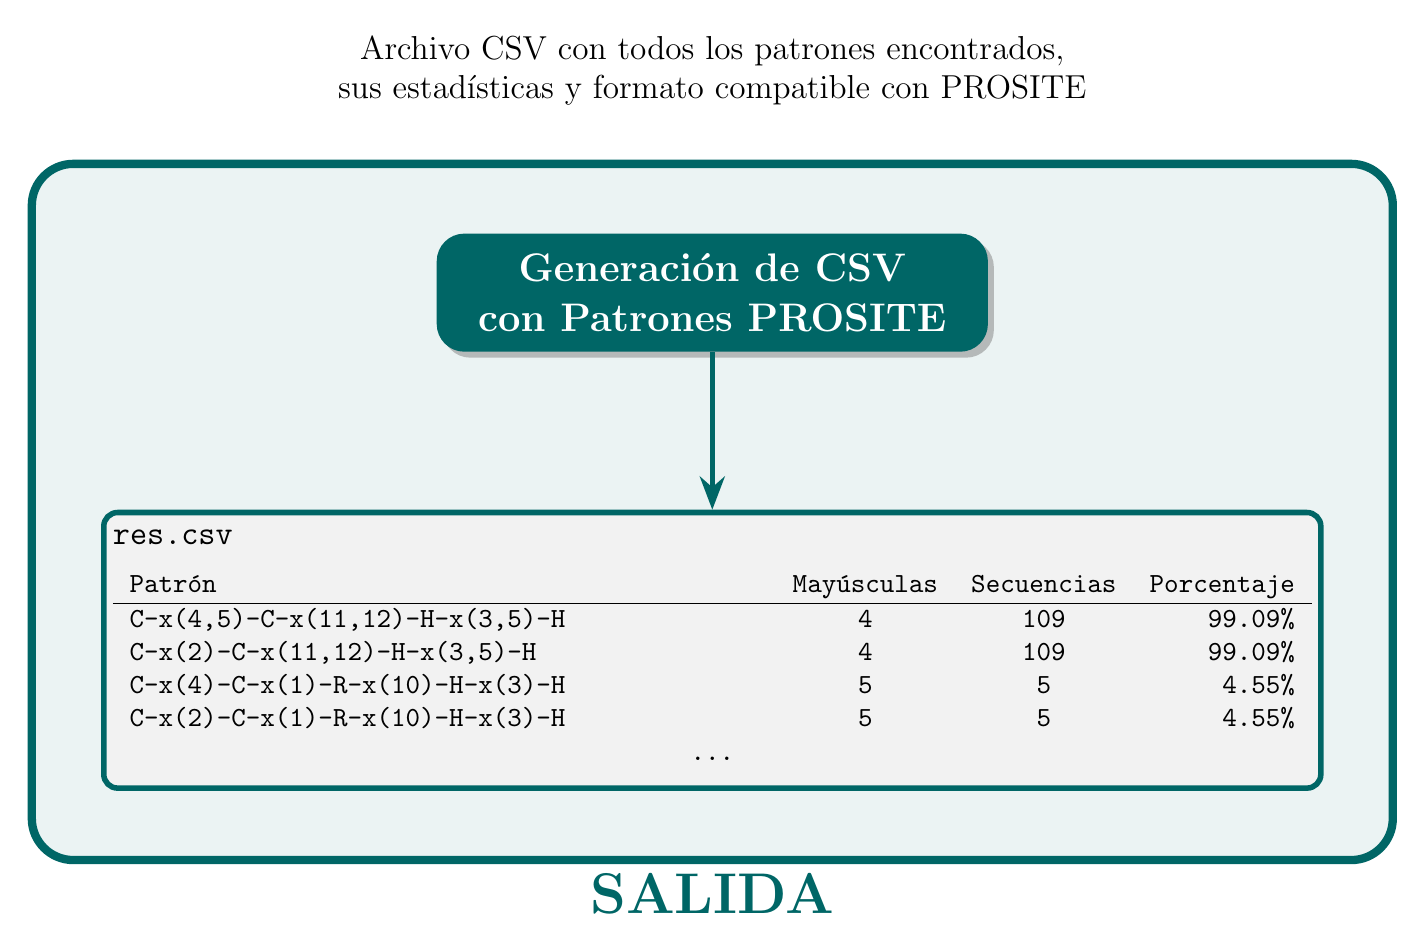
\begin{tikzpicture}[
        node distance=1.5cm,
        % Estilos para nodos principales
        mainbox/.style={
                rectangle,
                rounded corners=10pt,
                minimum width=7cm,
                minimum height=1.5cm,
                text centered,
                text width=6.5cm,
                font=\bfseries\Large,
                text=white,
                drop shadow
            },
        % Estilo para archivo CSV
        csvfile/.style={
                rectangle,
                rounded corners=5pt,
                minimum width=12cm,
                minimum height=3.5cm,
                text centered,
                font=\ttfamily\normalsize,
                text=black,
                fill=gray!10,
                draw=teal!80!black,
                line width=2pt,
                align=left
            },
        % Flechas
        arrow/.style={
                ->,
                >=Stealth,
                line width=2pt,
                color=teal!80!black
            },
        % Grupo contenedor
        groupbox/.style={
                rectangle,
                rounded corners=15pt,
                draw=teal!80!black,
                line width=3pt,
                fill=teal!80!black!8,
                inner sep=25pt
            }
    ]

    % Título principal
    \node[mainbox, fill=teal!80!black] (traduccion) {Generación de CSV\\con Patrones PROSITE};

    % CSV
    \node[csvfile, below=2cm of traduccion] (csv) {
        \textbf{\large res.csv}\\[8pt]
        \begin{tabular}{p{8cm} c c r}
        \textbf{Patrón} & \textbf{Mayúsculas} & \textbf{Secuencias} & \textbf{Porcentaje} \\
        \hline
        C-x(4,5)-C-x(11,12)-H-x(3,5)-H & 4 & 109 & 99.09\% \\
        C-x(2)-C-x(11,12)-H-x(3,5)-H & 4 & 109 & 99.09\% \\
        C-x(4)-C-x(1)-R-x(10)-H-x(3)-H & 5 & 5 & 4.55\% \\
        C-x(2)-C-x(1)-R-x(10)-H-x(3)-H & 5 & 5 & 4.55\% \\
        \multicolumn{4}{c}{...} \\
        \end{tabular}
    };

    % Grupo salida
    \begin{scope}[on background layer]
        \node[groupbox, fit=(traduccion)(csv), label={[font=\bfseries\huge, text=teal!80!black]below:SALIDA}] (salida) {};
    \end{scope}

    % Flecha
    \draw[arrow] (traduccion.south) -- (csv.north);

    % Descripción
    \node[above=1.5cm of traduccion, text width=12cm, align=center, font=\large] {
        Archivo CSV con todos los patrones encontrados,\\
        sus estadísticas y formato compatible con PROSITE
    };

\end{tikzpicture}

\end{document}
